\documentclass[margin=2mm,convert={density=300,size=1920x1080,outext=.png}]{standalone}

\usepackage{tikz}
\usepackage{xcolor}

\newcommand{\len}{7}% x direction
\newcommand{\wlen}{4}% x direction for w
\newcommand{\bre}{7}% y direction
\newcommand{\hei}{4}% z direction
\newcommand{\splitw}{2.5}% for the box in behind
\newcommand{\splitF}{0.5}% for the box in behind
\newcommand{\frontcolor}{black!15!white}
\newcommand{\topcolor}{black!30!white}
\newcommand{\sidecolor}{black!45!white}

\begin{document}
    % 1st box
    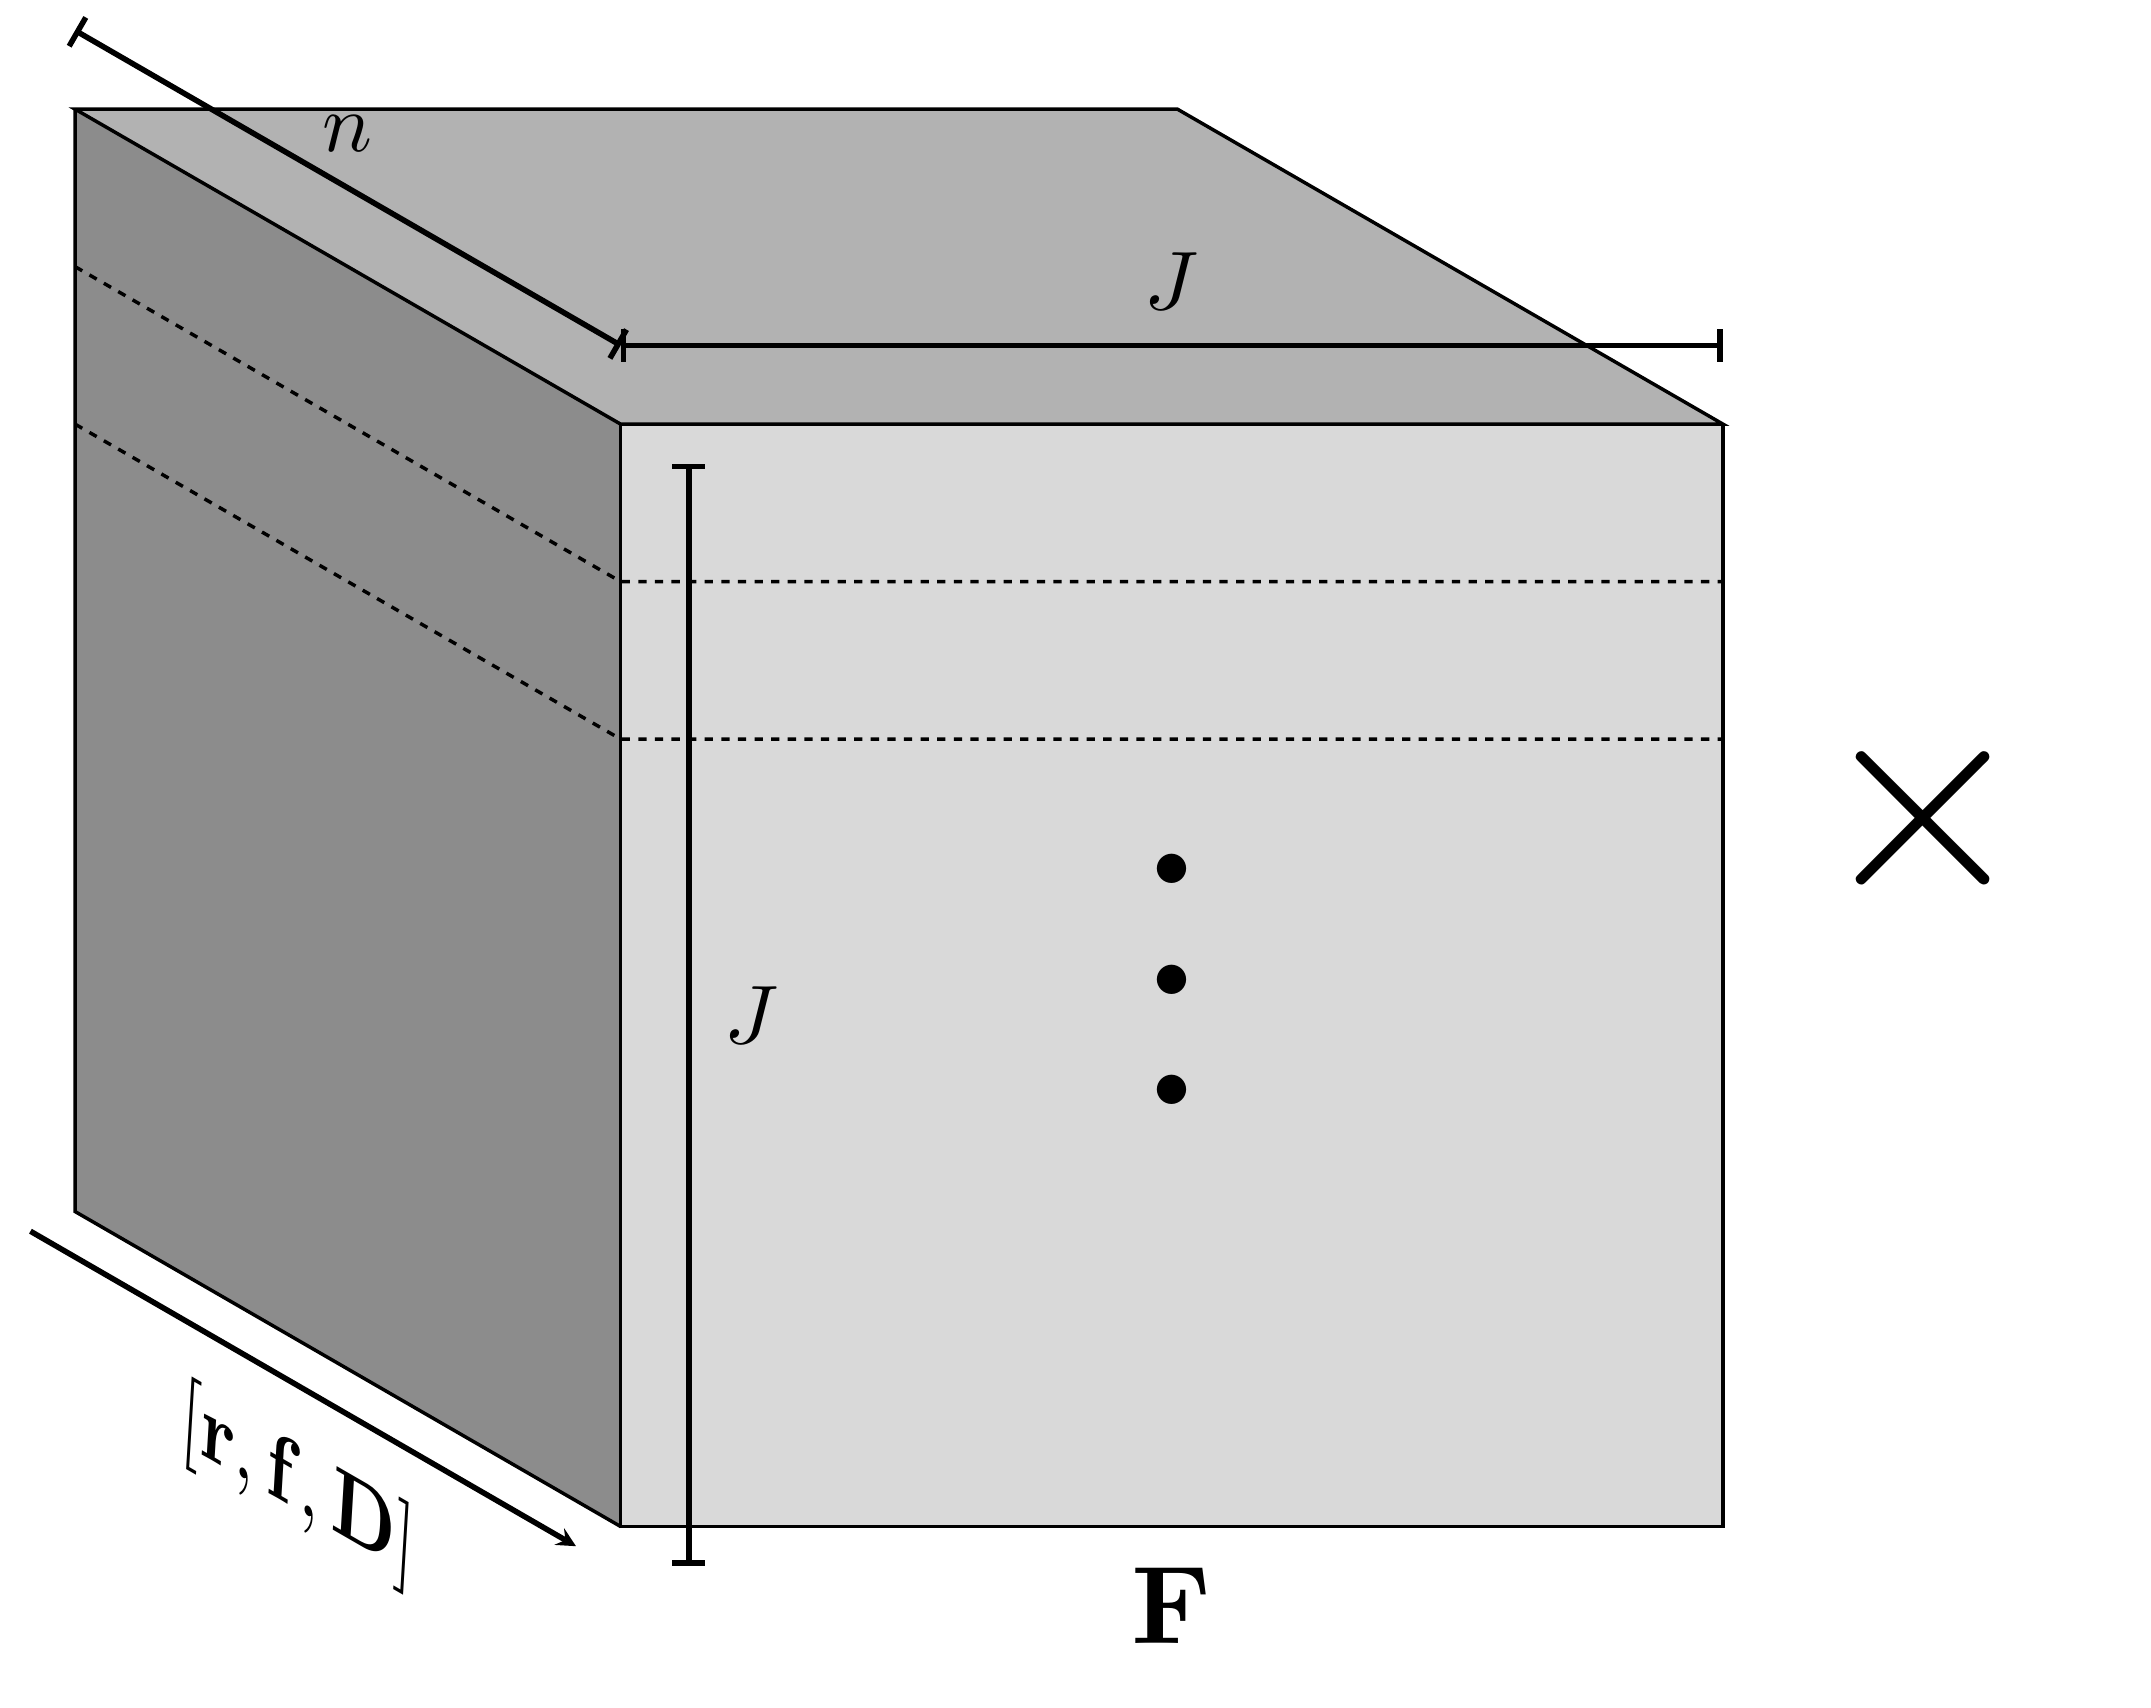
\begin{tikzpicture}[x=(0:2cm), y=(90:2cm), z=(330:2cm), >=stealth]
    \coordinate (O) at (0, 0, 0);
    \coordinate (A) at (\len, 0, 0);
    \coordinate (B) at (0, \bre, 0);
    \coordinate (C) at (\len, \bre, 0);
    \coordinate (D) at (0, 0, \hei);
    \coordinate (E) at (\len, 0, \hei);
    \coordinate (F) at (0, \bre, \hei);
    \coordinate (G) at (\len, \bre, \hei);
    
    % color
    \fill[\frontcolor] (D) -- (E) -- (G) -- (F) -- cycle;
    \fill[\topcolor] (B) -- (C) -- (G) -- (F) -- cycle;
    \fill[\sidecolor] (O) -- (B) -- (F) -- (D) -- cycle;
    
    % dotted lines
    \draw[dashed, line width=1.25pt] (0, \bre-1, 0) -- (0, \bre-1, \hei) -- (\len, \bre-1, \hei);
    \draw[dashed, line width=1.25pt] (0, \bre-2, 0) -- (0, \bre-2, \hei) -- (\len, \bre-2, \hei);
    \node [scale=10] at (\len/2, \bre-3, \hei) {$\vdots$};
    
    % box edges
    \draw[line width=1.25pt] (B) -- (F) -- (G) -- (C) -- cycle;
    \draw[line width=1.25pt] (F) -- (D) -- (E) -- (G);
    \draw[line width=1.25pt] (B) -- (O) -- (D);
    
    % labels
    \node [scale=4, rotate=0] at (\len/2, -.5, \hei) {$\mathbf{F}$};
    \draw [->, line width=2pt] (-.5, 0, .25) -- (-.5, 0, \hei+.25) node [midway, below=4pt, scale=3, rotate=330, xslant=-.5] {$[\mathbf{r}, \mathbf{f}, \mathbf{D}]$};
    \draw [|-|, line width=2pt] (0, \bre+.5, \hei) -- (\len, \bre+.5, \hei) node [midway, above, scale=3] {$J$};
    \draw [|-|, line width=2pt] (0, \bre+.5, 0) -- (0, \bre+.5, \hei) node [midway, above, scale=3] {$n$};
    \draw [|-|, line width=2pt] (0, \bre, \hei+.5) -- (0, 0, \hei+.5) node [midway, right, scale=3] {$J$};
    
    \node [scale=10] at (\len+3, \bre/2, \hei/2) {$\times$};
    \end{tikzpicture}
    % 2nd box
    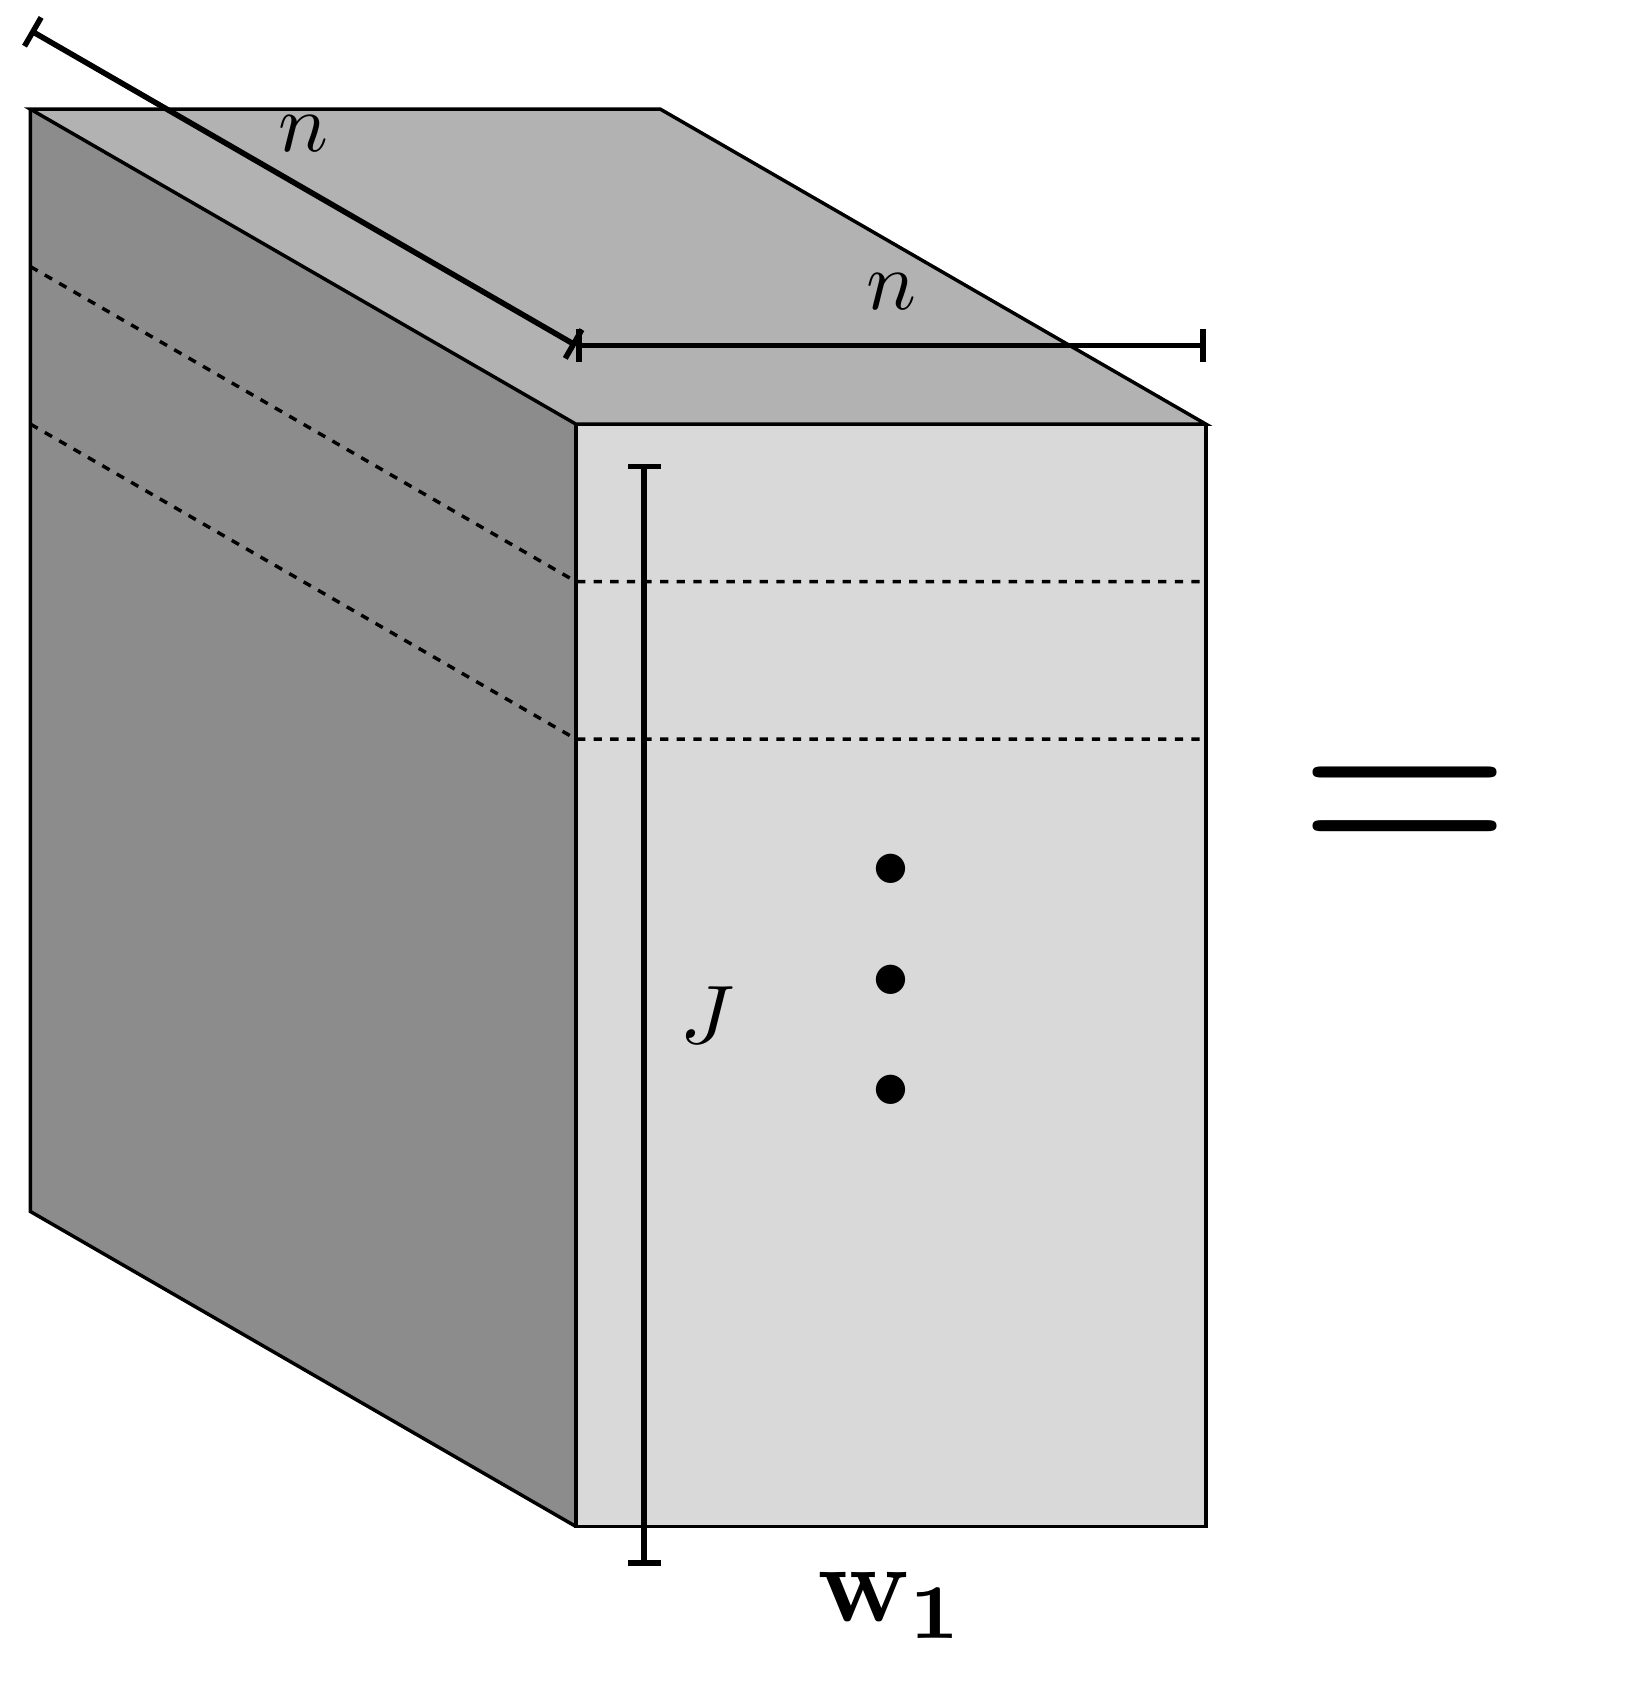
\begin{tikzpicture}[x=(0:2cm), y=(90:2cm), z=(330:2cm), >=stealth]
    \coordinate (O) at (0, 0, 0);
    \coordinate (A) at (\wlen, 0, 0);
    \coordinate (B) at (0, \bre, 0);
    \coordinate (C) at (\wlen, \bre, 0);
    \coordinate (D) at (0, 0, \hei);
    \coordinate (E) at (\wlen, 0, \hei);
    \coordinate (F) at (0, \bre, \hei);
    \coordinate (G) at (\wlen, \bre, \hei);
    
    % color
    \fill[\frontcolor] (D) -- (E) -- (G) -- (F) -- cycle;
    \fill[\topcolor] (B) -- (C) -- (G) -- (F) -- cycle;
    \fill[\sidecolor] (O) -- (B) -- (F) -- (D) -- cycle;
    
    % dotted lines
    \draw[dashed, line width=1.25pt] (0, \bre-1, 0) -- (0, \bre-1, \hei) -- (\wlen, \bre-1, \hei);
    \draw[dashed, line width=1.25pt] (0, \bre-2, 0) -- (0, \bre-2, \hei) -- (\wlen, \bre-2, \hei);
    \node [scale=10] at (\wlen/2, \bre-3, \hei) {$\vdots$};
    
    % box edges
    \draw[line width=1.25pt] (B) -- (F) -- (G) -- (C) -- cycle;
    \draw[line width=1.25pt] (F) -- (D) -- (E) -- (G);
    \draw[line width=1.25pt] (B) -- (O) -- (D);
    
    % labels
    \node [scale=4, rotate=0] at (\wlen/2, -.5, \hei) {$\mathbf{w_1}$};
    \draw [|-|, line width=2pt] (0, \bre+.5, \hei) -- (\wlen, \bre+.5, \hei) node [midway, above, scale=3] {$n$};
    \draw [|-|, line width=2pt] (0, \bre+.5, 0) -- (0, \bre+.5, \hei) node [midway, above, scale=3] {$n$};
    \draw [|-|, line width=2pt] (0, \bre, \hei+.5) -- (0, 0, \hei+.5) node [midway, right, scale=3] {$J$};
    
    \node [scale=10] at (\wlen+3, \bre/2, \hei/2) {$=$};
    \end{tikzpicture}
    % 3rd box
    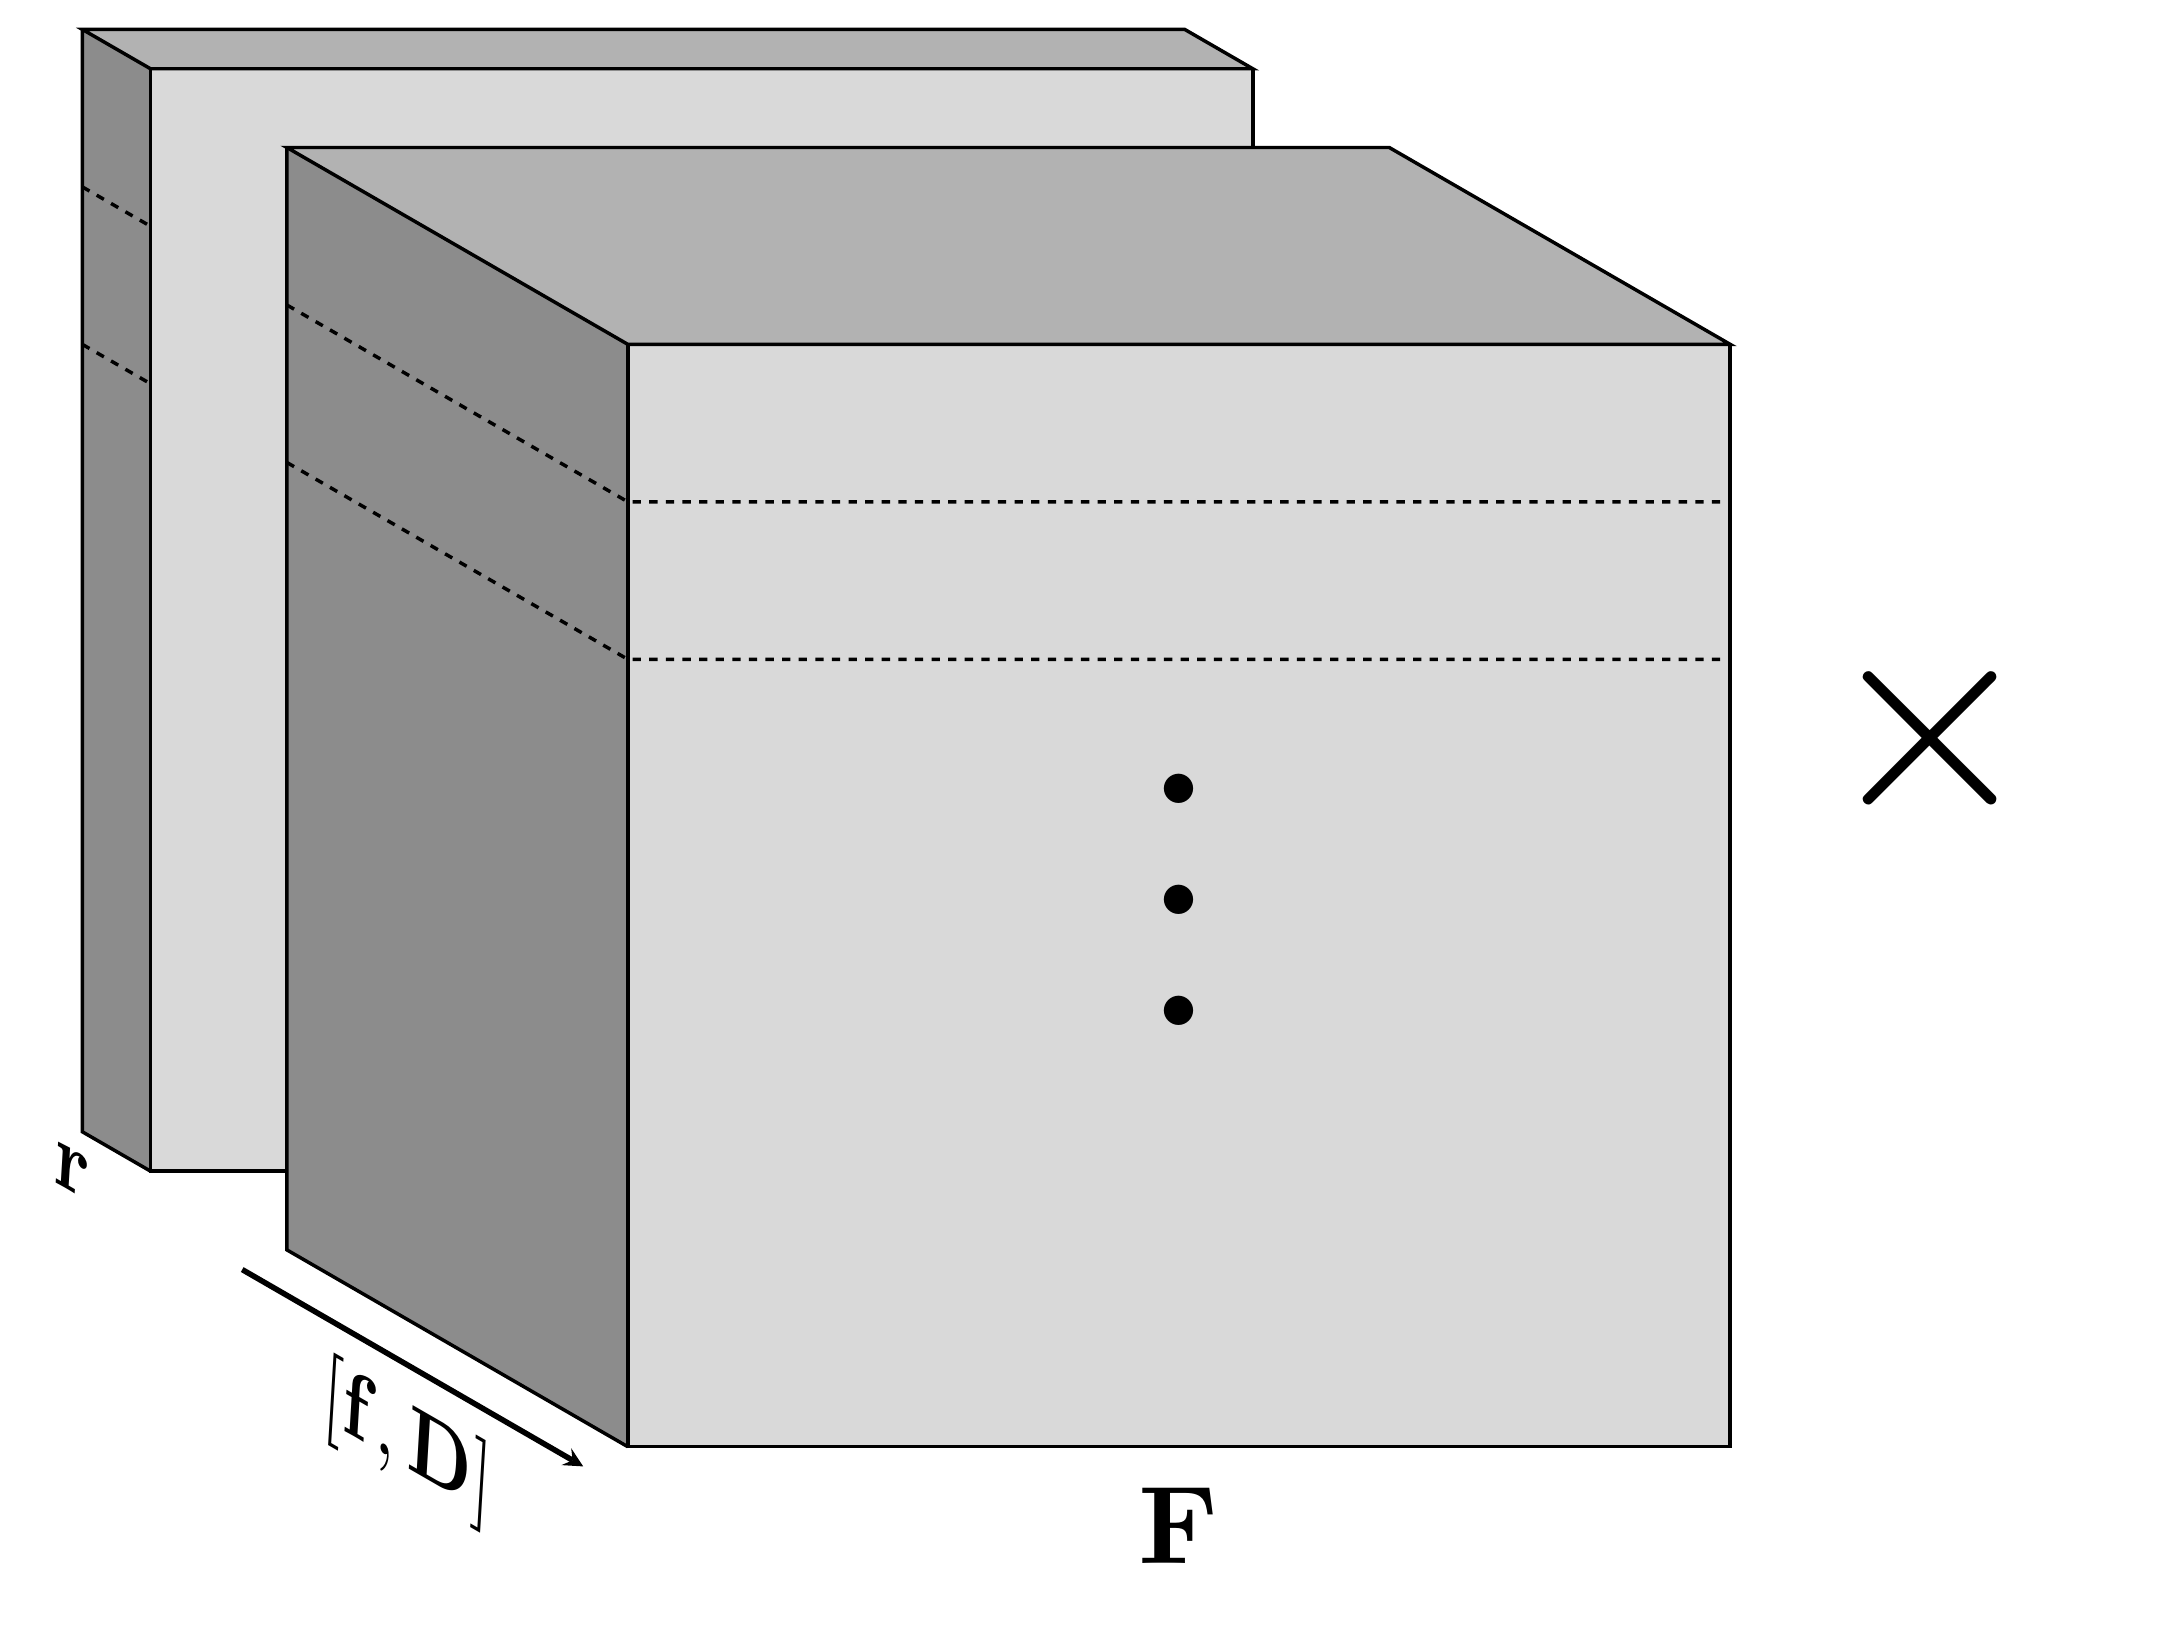
\begin{tikzpicture}[x=(0:2cm), y=(90:2cm), z=(330:2cm), >=stealth]
    \coordinate (backO) at (0, 0, 0);
    \coordinate (backA) at (\len, 0, 0);
    \coordinate (backB) at (0, \bre, 0);
    \coordinate (backC) at (\len, \bre, 0);
    \coordinate (backD) at (0, 0, \splitF);
    \coordinate (backE) at (\len, 0, \splitF);
    \coordinate (backF) at (0, \bre, \splitF);
    \coordinate (backG) at (\len, \bre, \splitF);
    
    % color
    \fill[\frontcolor] (backD) -- (backE) -- (backG) -- (backF) -- cycle;
    \fill[\topcolor] (backB) -- (backC) -- (backG) -- (backF) -- cycle;
    \fill[\sidecolor] (backO) -- (backB) -- (backF) -- (backD) -- cycle;
    
    % box edges
    \draw[line width=1.25pt] (backB) -- (backF) -- (backG) -- (backC) -- cycle;
    \draw[line width=1.25pt] (backF) -- (backD) -- (backE) -- (backG);
    \draw[line width=1.25pt] (backB) -- (backO) -- (backD);
    
    \coordinate (O) at (0, 0, \splitF+1);
    \coordinate (A) at (\len, 0, \splitF+1);
    \coordinate (B) at (0, \bre, \splitF+1);
    \coordinate (C) at (\len, \bre, \splitF+1);
    \coordinate (D) at (0, 0, \hei);
    \coordinate (E) at (\len, 0, \hei);
    \coordinate (F) at (0, \bre, \hei);
    \coordinate (G) at (\len, \bre, \hei);
    
    % color
    \fill[\frontcolor] (D) -- (E) -- (G) -- (F) -- cycle;
    \fill[\topcolor] (B) -- (C) -- (G) -- (F) -- cycle;
    \fill[\sidecolor] (O) -- (B) -- (F) -- (D) -- cycle;
    
    % dotted lines
    \draw[dashed, line width=1.25pt] (0, \bre-1, \splitF+1) -- (0, \bre-1, \hei) -- (\len, \bre-1, \hei);
    \draw[dashed, line width=1.25pt] (0, \bre-2, \splitF+1) -- (0, \bre-2, \hei) -- (\len, \bre-2, \hei);
    \node [scale=10] at (\len/2, \bre-3, \hei) {$\vdots$};
    
    % box edges
    \draw[line width=1.25pt] (B) -- (F) -- (G) -- (C) -- cycle;
    \draw[line width=1.25pt] (F) -- (D) -- (E) -- (G);
    \draw[line width=1.25pt] (B) -- (O) -- (D);
    
    % dotted lines
    \draw[dashed, line width=1.25pt] (0, \bre-1, 0) -- (0, \bre-1, \splitF);
    \draw[dashed, line width=1.25pt] (0, \bre-2, 0) -- (0, \bre-2, \splitF);
    
    % labels
    \node [scale=4, rotate=0] at (\len/2, -.5, \hei) {$\mathbf{F}$};
    \draw [->, line width=2pt] (-.5, 0, \splitF+1.25) -- (-.5, 0, \hei+.25) node [midway, below=-4pt, scale=3, rotate=330, xslant=-.5] {$[\mathbf{f}, \mathbf{D}]$};
    \node [scale=3, rotate=330, xslant=-.5] at (-.5, 0, .5) {$\mathbf{r}$};
    
    \node [scale=10] at (\len+3, \bre/2, \hei/2) {$\times$};
    \end{tikzpicture}
    % 4th box
    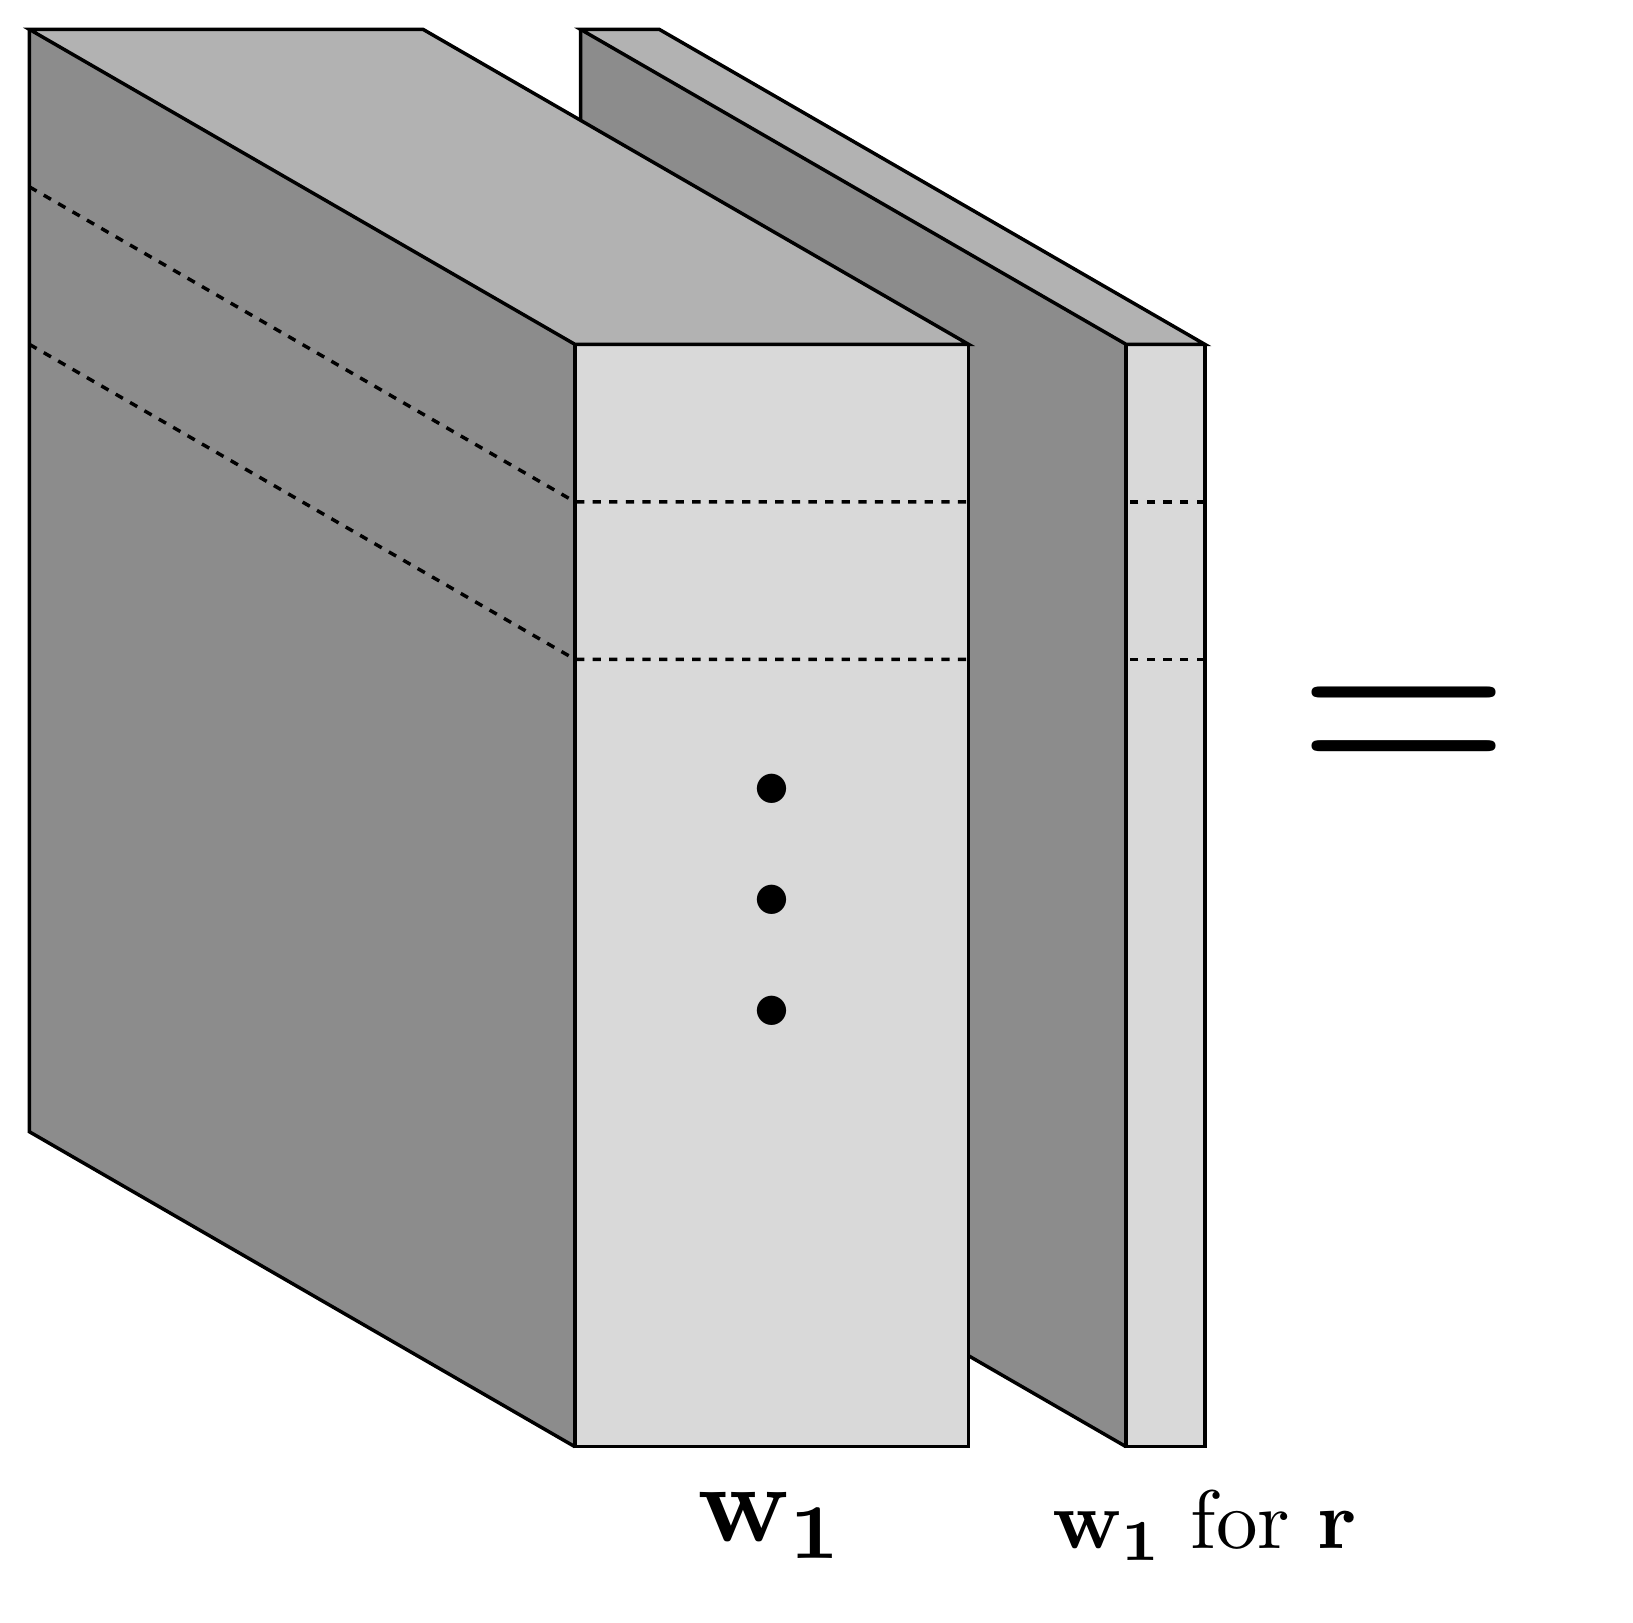
\begin{tikzpicture}[x=(0:2cm), y=(90:2cm), z=(330:2cm), >=stealth]
        \coordinate (splitO) at (0, 0, 0);
        \coordinate (splitA) at (\splitw, 0, 0);
        \coordinate (splitB) at (0, \bre, 0);
        \coordinate (splitC) at (\splitw, \bre, 0);
        \coordinate (splitD) at (0, 0, \hei);
        \coordinate (splitE) at (\splitw, 0, \hei);
        \coordinate (splitF) at (0, \bre, \hei);
        \coordinate (splitG) at (\splitw, \bre, \hei);
        
        \coordinate (O) at (\splitw+1, 0, 0);
        \coordinate (A) at (\wlen, 0, 0);
        \coordinate (B) at (\splitw+1, \bre, 0);
        \coordinate (C) at (\wlen, \bre, 0);
        \coordinate (D) at (\splitw+1, 0, \hei);
        \coordinate (E) at (\wlen, 0, \hei);
        \coordinate (F) at (\splitw+1, \bre, \hei);
        \coordinate (G) at (\wlen, \bre, \hei);
        
        % color
        \fill[\frontcolor] (D) -- (E) -- (G) -- (F) -- cycle;
        \fill[\topcolor] (B) -- (C) -- (G) -- (F) -- cycle;
        \fill[\sidecolor] (O) -- (B) -- (F) -- (D) -- cycle;
        
        % box edges
        \draw[line width=1.25pt] (B) -- (F) -- (G) -- (C) -- cycle;
        \draw[line width=1.25pt] (F) -- (D) -- (E) -- (G);
        \draw[line width=1.25pt] (B) -- (O) -- (D);
        
        % color
        \fill[\frontcolor] (splitD) -- (splitE) -- (splitG) -- (splitF) -- cycle;
        \fill[\topcolor] (splitB) -- (splitC) -- (splitG) -- (splitF) -- cycle;
        \fill[\sidecolor] (splitO) -- (splitB) -- (splitF) -- (splitD) -- cycle;
        
        % dotted lines
        \draw[dashed, line width=1.25pt] (0, \bre-1, 0) -- (0, \bre-1, \hei) -- (\splitw, \bre-1, \hei);
        \draw[dashed, line width=1.25pt] (0, \bre-2, 0) -- (0, \bre-2, \hei) -- (\splitw, \bre-2, \hei);
        \node [scale=10] at (\splitw/2, \bre-3, \hei) {$\vdots$};
        
        % box edges
        \draw[line width=1.25pt] (splitB) -- (splitF) -- (splitG) -- (splitC) -- cycle;
        \draw[line width=1.25pt] (splitF) -- (splitD) -- (splitE) -- (splitG);
        \draw[line width=1.25pt] (splitB) -- (splitO) -- (splitD);
        
        % dotted lines
        \draw[dashed, line width=1.25pt] (\wlen, \bre-1, \hei) -- (\splitw+1, \bre-1, \hei);
        \draw[dashed, line width=1.25pt] (\wlen, \bre-2, \hei) -- (\splitw+1, \bre-2, \hei);
        
        % labels
        \node [scale=4, rotate=0] at (\splitw/2, -.5, \hei) {$\mathbf{w_1}$};
        \node [scale=3, rotate=0] at (\splitw+1.5, -.5, \hei) {$\mathbf{w_1}$ for $\mathbf{r}$};
        
        \node [scale=10] at (\wlen+3, \bre/2, \hei/2) {$=$};
    \end{tikzpicture}
    % 5th box
    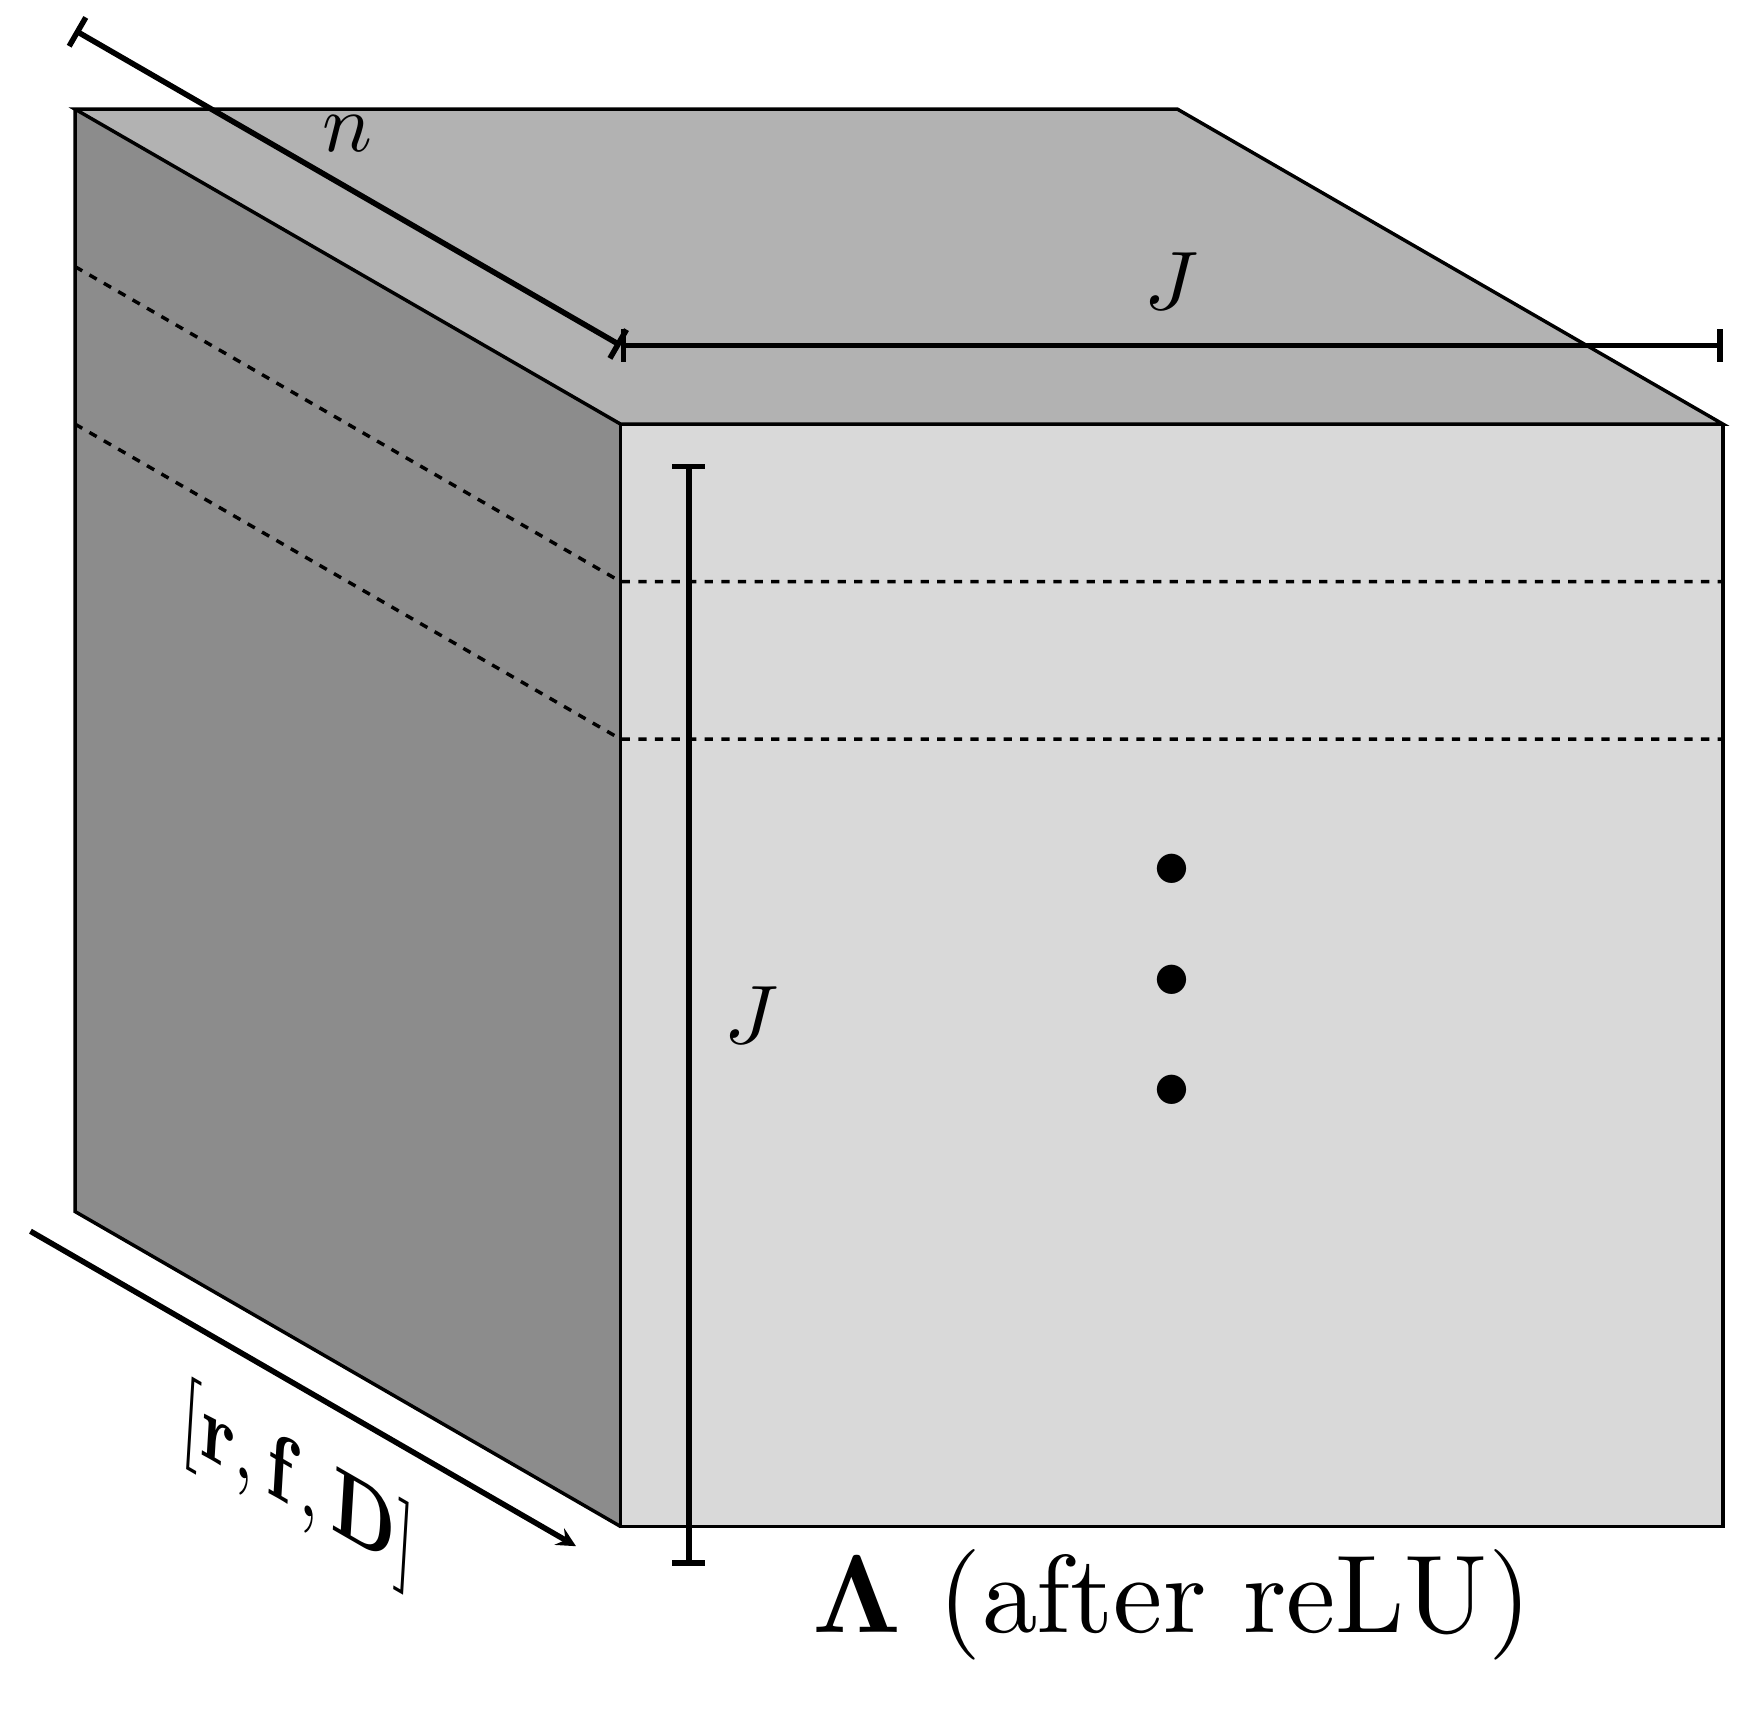
\begin{tikzpicture}[x=(0:2cm), y=(90:2cm), z=(330:2cm), >=stealth]
    \coordinate (O) at (0, 0, 0);
    \coordinate (A) at (\len, 0, 0);
    \coordinate (B) at (0, \bre, 0);
    \coordinate (C) at (\len, \bre, 0);
    \coordinate (D) at (0, 0, \hei);
    \coordinate (E) at (\len, 0, \hei);
    \coordinate (F) at (0, \bre, \hei);
    \coordinate (G) at (\len, \bre, \hei);
    
    % color
    \fill[\frontcolor] (D) -- (E) -- (G) -- (F) -- cycle;
    \fill[\topcolor] (B) -- (C) -- (G) -- (F) -- cycle;
    \fill[\sidecolor] (O) -- (B) -- (F) -- (D) -- cycle;
    
    % dotted lines
    \draw[dashed, line width=1.25pt] (0, \bre-1, 0) -- (0, \bre-1, \hei) -- (\len, \bre-1, \hei);
    \draw[dashed, line width=1.25pt] (0, \bre-2, 0) -- (0, \bre-2, \hei) -- (\len, \bre-2, \hei);
    \node [scale=10] at (\len/2, \bre-3, \hei) {$\vdots$};
    
    % box edges
    \draw[line width=1.25pt] (B) -- (F) -- (G) -- (C) -- cycle;
    \draw[line width=1.25pt] (F) -- (D) -- (E) -- (G);
    \draw[line width=1.25pt] (B) -- (O) -- (D);
    
    % labels
    \node [scale=4, rotate=0] at (\len/2, -.5, \hei) {$\mathbf{\Lambda}$ (after reLU)};
    \draw [->, line width=2pt] (-.5, 0, .25) -- (-.5, 0, \hei+.25) node [midway, below=4pt, scale=3, rotate=330, xslant=-.5] {$[\mathbf{r}, \mathbf{f}, \mathbf{D}]$};
    \draw [|-|, line width=2pt] (0, \bre+.5, \hei) -- (\len, \bre+.5, \hei) node [midway, above, scale=3] {$J$};
    \draw [|-|, line width=2pt] (0, \bre+.5, 0) -- (0, \bre+.5, \hei) node [midway, above, scale=3] {$n$};
    \draw [|-|, line width=2pt] (0, \bre, \hei+.5) -- (0, 0, \hei+.5) node [midway, right, scale=3] {$J$};
    \end{tikzpicture}
    asdf
\end{document}